\begin{frame}[label=title]
    \centering
    \begin{figure}[H]
        
\includegraphics[keepaspectratio, width=0.7\paperwidth, height=\paperheight]{LeeLogo}
    \end{figure}
    Informatik: Data Science und Sicherheit\\
    \textbf{Lektion 4} \emoji{computer}: \textbf{Geheimschriften}
\end{frame}

\begin{frame}{Inhalt}
    \begin{itemize}
        \item \emoji{nerd-face} Weshalb Verschlüsselung?
        \item \emoji{thinking-face} Anforderungen an Verschlüsselungsverfahren
        \item \emoji{key} Symmetrische Verschlüsselungsverfahren
        %\item \emoji{chart-increasing} Häufigkeitsanalyse
    \end{itemize}
\end{frame}

\begin{frame}{Weshalb Verschlüsselung?}
\begin{itemize}
    \item Sie wollen einander etwas schreiben, ohne dass ich es mitlesen kann
    \item Sie wollen einander ein Bild schicken, ohne dass Ihre Eltern es sehen können
    \item Sie wollen etwas kaufen, ohne ihre Bankkonto-Daten an fremde Personen preiszugeben
\end{itemize}


    
\end{frame}

\begin{frame}{Weshalb Verschlüsselung?}
    \begin{figure}[H]
        
\includegraphics[keepaspectratio, width=0.49\linewidth]{GrundlagenInfo/DataScience/03_Kryptologie/Figures/encryption-example-1.png}
        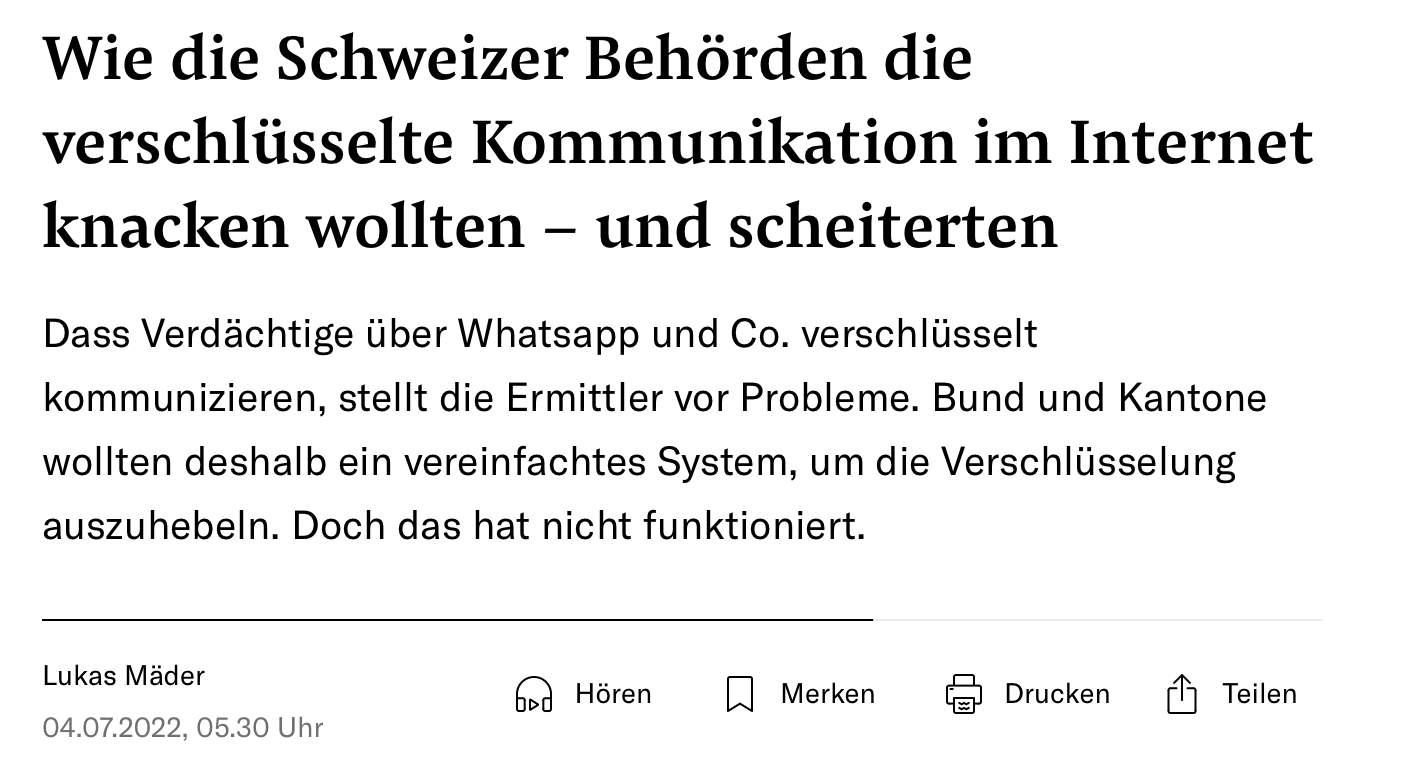
\includegraphics[keepaspectratio, width=0.49\linewidth]{GrundlagenInfo/DataScience/03_Kryptologie/Figures/encryption-example-2.png}
        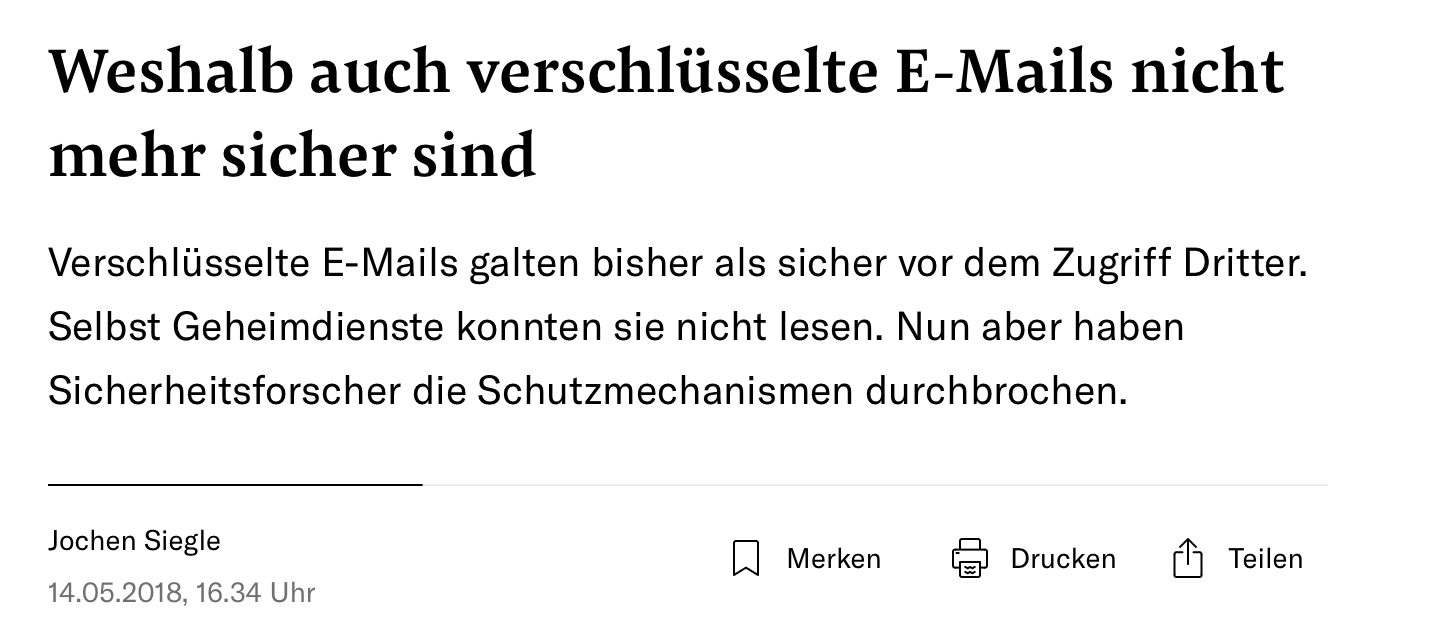
\includegraphics[keepaspectratio, width=0.6\linewidth]{GrundlagenInfo/DataScience/03_Kryptologie/Figures/encryption-example-3.png}
    \end{figure}
\end{frame}

\begin{frame}[label=schemakrypto]{Schematische Darstellung der Kommunikation zwischen Bob und Alice}
\begin{figure}
    \centering
    \begin{tikzpicture}[mylabel/.style={text width=20mm, align=center},scale=0.8, every node/.style={scale=0.8}]
    \node[bob, minimum width=1.5cm, 
        label={[mylabel, anchor=west]north east:{}}, 
        label={[mylabel, anchor=east]north west:{\textcolor{Blue}{Klartext} $\big\downarrow\text{\tiny (Verschlüsselung)}$\\
        \textcolor{Red}{Geheimtext}}}] (bob) {Bob (Sender)};
    \node[alice, minimum width=1.5cm, right=5cm of bob, mirrored,
        label={[mylabel, anchor=east]north west:{}}, 
        label={[mylabel, anchor=west]north east:{\textcolor{Red}{Geheimtext} $\big\downarrow\text{\tiny (Entschlüsselung)}$\\
        \textcolor{Blue}{Klartext}}}] (alice) {Alice (Empfänger)};
    
    \draw[->, thick, black] ([yshift=0mm]bob.east) coordinate(aux-a)-- coordinate[near start] (aux) node[above, text width=3cm, align=center]{\textcolor{Red}{Geheimtext}} (aux-a-|alice.west);

    \node[devil, minimum width=1.5cm, below right=13mm and 1.6cm of bob] (eve) {Eve (Gegner / Abhörer)};
    \draw[<-, gray] (eve)--(aux) node[midway,right]{abhören};
    \end{tikzpicture}
    \\[1cm]$\rightarrow$ Vertraulichkeit, Integrität, Authentizität, Verbindlichkeit
\end{figure}
\end{frame}

\begin{frame}{Anforderungen an kryptographische Systeme}
\begin{enumerate}[<+->]
    \item \textbf{Vertraulichkeit}: Es soll sichergestellt sein, dass wirklich nur diejenige eine Nachricht lesen kann, für die diese bestimmt ist.
    \item \textbf{Integrität}: Die Empfängerin soll feststellen können, ob die Nachricht nach ihrer Erzeugung verändert wurde.
    \item \textbf{Authentizität} Der Verfasser einer Nachricht soll identifizierbar sein, bzw. die Empfängerin soll nachprüfen können, wer der Verfasser ist.
    \item \textbf{Verbindlichkeit}: Der Verfasser soll nicht abstreiten können, dass er der Verfasser der Nachricht ist.
\end{enumerate}
\end{frame}

\begin{frame}{Symmetrische Verschlüsselungsverfahren}
    \begin{itemize}[<+->]
        \item \emoji{key} Derselbe Schlüssel zur Ver- und Entschlüsselung
        \item \emoji{shushing-face} Sender und Empfänger müssen sich auf einen Schlüssel einigen, ohne dass ein Dritter mithören kann
        \item \emoji{locked-with-key} Analogie: Schatzkiste versenden
    \end{itemize}

\end{frame}

\begin{frame}[label=intro1]{Einführungsaufgabe}
    Der Geheimtext lautet:
    \begin{center}
        AMEHT SEGITHCIW NIE TSI EIGOLOTPYRK
    \end{center}
    Stellen Sie den ursprünglichen Text wieder her.
\end{frame}

\begin{frame}[label=intro1Sol]{Lösung der Einführungsaufgabe}
    \begin{center}
    
        Geheimtext:\\
        AMEHT SEGITHCIW NIE TSI EIGOLOTPYRK\\
        \bigskip
        ursprünglicher Text:\\
        KRYPTOLOGIE IST EIN WICHTIGES THEMA\\
    \end{center}
    Der Geheimtext entspricht dem von rechts nach links (rückwärts) gelesenen ursprünglichen Text.
\end{frame}

\begin{frame}[label=intro2]{Einführungsaufgabe (Aufgabe 2.1)}
    Der Geheimtext lautet:
    \begin{center}
    \small
        \begin{enumerate}
            \item RKPYOTOLIGEEMREOLGCITHEGEHMIINSSE
            \item HCSFIRILTAHCZFUEBUHAWNERDNUKUZMMOINUEIZNER
        \end{enumerate}
        \normalsize
    \end{center}
    Stellen Sie den ursprünglichen Text wieder her.
\end{frame}

\begin{frame}[label=intro2Sol]{Lösung Einführungsaufgabe (Aufgabe 2.1)}
    Geheimtext:
    \begin{center}
    \small
        \begin{enumerate}
            \item RKPYOTOLIGEEMREOLGCITHEGEHMIINSSE
            \item HCSFIRILTAHCZFUEBUHAWNERDNUKUZMMOINUEIZNER
        \end{enumerate}
        \normalsize
    \end{center}
    Ursprünglicher Text:
    \begin{center}
    \small
        \begin{enumerate}
            \item KRYPTOLOGIE ERMOEGLICHT GEHEIMNISSE
            \item SCHRIFTLICH AUFZUBEWAHREN UND ZU KOMMUNIZIEREN
        \end{enumerate}
        \normalsize
    \end{center}
    Der Geheimtext entsteht durch Austauschen der Positionen der Buchstaben.
    \begin{figure}[H]
        \centering
        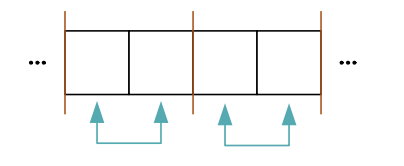
\includegraphics[width=0.4\linewidth]{GrundlagenInfo/DataScience/03_Kryptologie/Figures/krypto_swap_2.png}
        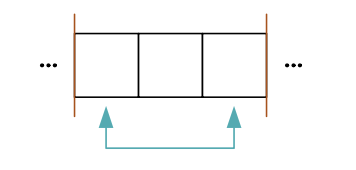
\includegraphics[width=0.35\linewidth]{GrundlagenInfo/DataScience/03_Kryptologie/Figures/krypto_swap_3.png}
    \end{figure}
\end{frame}

\begin{frame}[label=intro]{Einführungsaufgabe Skytale}
    
\end{frame}

\begin{frame}[fragile, label=sol22]{Teillösung der Aufgabe 2.2}
\begin{lstlisting}[style=TigerJython, basicstyle=\scriptsize]
def zweiertausch(klartext):
    geheimtext = ""
    b = 0
    while b < (len(klartext) - 1):
        geheimtext += klartext[b + 1] + klartext[b]
        b += 2

    if len(klartext) % 2 != 0:
        # Klartexte ungerader Länge
        geheimtext += klartext[len(klartext) - 1]
    print(geheimtext)


zweiertausch("KANTONSSCHULE")
\end{lstlisting}
\end{frame}

\section{Chiffrierung mit Hilfe von Tabellen}

\begin{frame}[label=skytale1]{SKYTALE}
\begin{itemize}
    \item Schreibe den Klartext zeilenweise in eine Tabelle (Matrix) von links nach rechts.
    \item Der Geheimtext erhalten wir, indem wir die Buchstaben Spalte für Spalte von links nach rechts lesen.
\end{itemize}
\begin{table}[]
\begin{tabular}{|c|c|c|c|c|c|c|}
\hline
\blue{S} & P & A & R & T & A & \blue{W} \\ \hline
A & R & \blue{I} & N & \blue{D} & E & R \\ \hline
\blue{A} & N & T & I & K & E & \blue{D} \\ \hline
E & R & \blue{H} & A & U & P & T \\ \hline
O & R & T & \blue{D} & E & R & \blue{L} \\ \hline
A & N & D & S & C & H & A \\ \hline
F & T & \blue{L} & A & K & O & N \\ \hline
I & E & N & \red{X} & \red{K} & \red{M} & \red{G} \\ \hline
\end{tabular}
\end{table}
\end{frame}

\begin{frame}[label=skytale2]{SKYTALE}
\begin{itemize}
    \item Falls der Klartext die Tabelle nicht vollständig ausfüllt, so füllt man die leeren Felder mit beliebigen Buchstaben auf (rot markiert).
\end{itemize}
\begin{table}[]
\begin{tabular}{|c|c|c|c|c|c|c|}
\hline
\blue{S} & P & A & R & T & A & \blue{W} \\ \hline
A & R & \blue{I} & N & \blue{D} & E & R \\ \hline
\blue{A} & N & T & I & K & E & \blue{D} \\ \hline
E & R & \blue{H} & A & U & P & T \\ \hline
O & R & T & \blue{D} & E & R & \blue{L} \\ \hline
A & N & D & S & C & H & A \\ \hline
F & T & \blue{L} & A & K & O & N \\ \hline
I & E & N & \red{X} & \red{K} & \red{M} & \red{G} \\ \hline
\end{tabular}
\end{table}
\end{frame}

\begin{frame}[label=skytaleEx1]{SKYTALE Aufgabe 1}
Die Geheimschrift
\begin{center}
    WNGIAEIEMATSMKRTTEAGIEINANINTUGNDOJEEENL
\end{center}
wurde mit einer Tabelle mit 5 Zeilen und 8 Spalten erzeugt. Wie lautet der Klartext?
\end{frame}

\begin{frame}[label=skytaleEx1Sol]{Lösung SKYTALE Aufgabe 1}
Wir beginnen mit einer leeren $5\times 8$ Tabelle und schreiben den Geheimtext spaltenweise (von rechts nach links und von oben nach unten) in die leere Tabelle. Damit erhalten wir:
\begin{table}[]
\begin{tabular}{|c|c|c|c|c|c|c|c|}
\hline
W & E & T & T & I & N & G & E \\ \hline
N & I & S & T & E & I & N & E \\ \hline
G & E & M & E & I & N & D & E \\ \hline
I & M & K & A & N & T & O & N \\ \hline
A & A & R & G & A & U & \red{J} & \red{L} \\ \hline
\end{tabular}
\end{table}
Der Klartext
\begin{center}
    Wettingen ist eine Gemeinde im Kanton Aargau
\end{center}
lässt sich nun einfach ablesen.
\end{frame}

\begin{frame}[label=skytaleEx2]{SKYTALE Aufgabe 2}
Sie möchten einen Klartext der Länge 87 mit Hilfe einer Tabelle mit 10 Zeilen chiffrieren. Wie viele Spalten benötigt diese Tabelle?
\end{frame}

\begin{frame}[label=skytaleEx2Sol]{Lösung SKYTALE Aufgabe 2}
Die Tabelle benötigt 9 Spalten. Allgemein lässt sich die Anzahl benötigter Spalten berechnen durch
\begin{align*}
    \ceil{\frac{\text{Länge des Textes}}{\text{Anzahl Zeilen}}}\quad\text{(nach oben aufgerundet)}.
\end{align*}
\end{frame}

\begin{frame}[label=skytaleEx3]{SKYTALE Aufgabe 3}
Der folgende Geheimtext der Länge 75 wurde mit SKYTALE verschlüsselt:
\begin{center}
ETIFIITNUTNFGENKURRELEODIERSILIMSEANIE\\
MRECREMRHSNSSAPSTCBRCRHEUHORRNHNIEGEG 
\end{center}
Dabei konnten \textbf{alle Zeilen der Tabelle vollständig aufgefüllt} werden.
\begin{description}
\item[(a)] Welches ist hier der Schlüssel (die Anzahl der Zeilen)? Tipp: Probieren Sie die Schlüssel 3 und 5 aus.
\item[(b)] Wie lautet der Klartext?
\item[(c)] Wie viele Schlüssel müssen im schlimmsten Fall ausprobiert werden, bis der korrekte Schlüssel gefunden wurde? Das heisst, wie viele potentielle Schlüssel gibt es?
\end{description}
\end{frame}

\begin{frame}[fragile, label=skytaleEx3Sol]{Lösung SKYTALE Aufgabe 3}
% \adjustbox{width=0.7\textwidth}{%
\begin{table}[]
\begin{tabular}{|c|c|c|c|c|c|c|c|c|c|c|c|c|c|c|}
\hline
E & I & N & K & L & E & I & N & E & R & S & C & H & R & I \\ \hline
T & T & F & U & E & R & M & I & C & H & A & B & E & R & E \\ \hline
I & N & G & R & O & S & S & E & R & S & P & R & U & N & G \\ \hline
F & U & E & R & D & I & E & M & E & N & S & C & H & H & E \\ \hline
I & T & N & E & I & L & A & R & M & S & T & R & O & N & G \\ \hline
\end{tabular}
\end{table}
% }%
\begin{description}
\item[(a)] Durch Ausprobieren finden wir, dass die Wahl des Schlüssels 5 zu einem sinnvollen Klartext führt, die Wahl des Schlüssels 3 jedoch nicht.

\item[(b)]
Der Klartext lautet also:
\begin{center}
    {\small
    EIN KLEINER SCHRITT FUER MICH ABER EIN GROSSER\\
    SPRUNG FUER DIE MENSCHHEIT NEIL ARMSTRONG}
\end{center}
\item[(c)] Wir müssen $75=3\cdot 5\cdot 5$ Buchstaben auf ein Rechteck verteilen. Damit könnten $3, 5, 15$ und $25$ mögliche Schlüssel sein. $1$ und $75$ sind keine Schlüssel, da der gegebene Text kein Klartext ist.
\end{description}
\end{frame}

\section{Richelieu}

\begin{frame}[label=richelieu]{RICHELIEU}
\begin{table}[]
\scalebox{0.7}{%
\begin{tabular}{|c|c|c|c|c|}
\hline
H & I & B & E & N \\ \hline
V & F & O & F & Q \\ \hline
R & E & M & T & A \\ \hline
N & O & T & L & I \\ \hline
U & K & G & A & N \\ \hline
\end{tabular}}
%\caption*{Kryptotext}
\end{table}



\begin{table}[]
\scalebox{0.7}{%
\begin{tabular}{|c|c|c|
>{\columncolor[HTML]{9B9B9B}}c |c|}
\hline
\cellcolor[HTML]{9B9B9B}{\color[HTML]{9B9B9B} H} & {\color[HTML]{FFFFFF} I}                         & \cellcolor[HTML]{9B9B9B}{\color[HTML]{9B9B9B} B} & {\color[HTML]{9B9B9B} E} & {\color[HTML]{FFFFFF} N}                         \\ \hline
\cellcolor[HTML]{9B9B9B}{\color[HTML]{9B9B9B} V} & {\color[HTML]{FFFFFF} F}                         & {\color[HTML]{FFFFFF} O}                         & {\color[HTML]{9B9B9B} F} & \cellcolor[HTML]{9B9B9B}{\color[HTML]{9B9B9B} Q} \\ \hline
{\color[HTML]{FFFFFF} R}                         & \cellcolor[HTML]{9B9B9B}{\color[HTML]{9B9B9B} E} & {\color[HTML]{FFFFFF} M}                         & {\color[HTML]{9B9B9B} T} & {\color[HTML]{FFFFFF} A}                         \\ \hline
\cellcolor[HTML]{9B9B9B}{\color[HTML]{9B9B9B} N} & \cellcolor[HTML]{9B9B9B}{\color[HTML]{9B9B9B} O} & {\color[HTML]{FFFFFF} T}                         & {\color[HTML]{9B9B9B} L} & {\color[HTML]{FFFFFF} I}                         \\ \hline
\cellcolor[HTML]{9B9B9B}{\color[HTML]{9B9B9B} U} & {\color[HTML]{FFFFFF} K}                         & \cellcolor[HTML]{9B9B9B}{\color[HTML]{9B9B9B} G} & {\color[HTML]{9B9B9B} A} & \cellcolor[HTML]{9B9B9B}{\color[HTML]{9B9B9B} N} \\ \hline
\end{tabular}}
%\caption*{Schlüssel}
\end{table}



\begin{table}[]
\scalebox{0.7}{%
\begin{tabular}{|c|c|c|
>{\columncolor[HTML]{9B9B9B}}c |c|}
\hline
\cellcolor[HTML]{9B9B9B}{\color[HTML]{9B9B9B} H} & {\color[HTML]{000000} I}                         & \cellcolor[HTML]{9B9B9B}{\color[HTML]{9B9B9B} B} & {\color[HTML]{9B9B9B} E} & {\color[HTML]{000000} N}                         \\ \hline
\cellcolor[HTML]{9B9B9B}{\color[HTML]{9B9B9B} V} & {\color[HTML]{000000} F}                         & {\color[HTML]{000000} O}                         & {\color[HTML]{9B9B9B} F} & \cellcolor[HTML]{9B9B9B}{\color[HTML]{9B9B9B} Q} \\ \hline
{\color[HTML]{000000} R}                         & \cellcolor[HTML]{9B9B9B}{\color[HTML]{9B9B9B} E} & {\color[HTML]{000000} M}                         & {\color[HTML]{9B9B9B} T} & {\color[HTML]{000000} A}                         \\ \hline
\cellcolor[HTML]{9B9B9B}{\color[HTML]{9B9B9B} N} & \cellcolor[HTML]{9B9B9B}{\color[HTML]{9B9B9B} O} & {\color[HTML]{000000} T}                         & {\color[HTML]{9B9B9B} L} & {\color[HTML]{000000} I}                         \\ \hline
\cellcolor[HTML]{9B9B9B}{\color[HTML]{9B9B9B} U} & {\color[HTML]{000000} K}                         & \cellcolor[HTML]{9B9B9B}{\color[HTML]{9B9B9B} G} & {\color[HTML]{9B9B9B} A} & \cellcolor[HTML]{9B9B9B}{\color[HTML]{9B9B9B} N} \\ \hline
\end{tabular}}
%\caption*{Klartext}
\end{table}
\end{frame}

\begin{frame}[fragile, label=binSchloss]{Binäres Zahlenschloss}
Zahlenschloss mit 4 Stellen. An jeder Stelle kann entweder eine 0 oder eine 1 gewählt werden.
\begin{center}
\begin{forest}
  for tree={
    draw=gray,
    circle,
    fill=gray,
    s sep'+=5pt,
    inner sep=.75pt,
  },
  label me/.style={
    edge label={node [midway,inner sep=1pt,above,sloped,font=\footnotesize] {$#1$}},
  },
  tikz+={
    \draw [-Latex, gray] (.north west) ++(-15pt,15pt) -- ++(-25pt,0) node [midway, above, anchor=west, font=\footnotesize, inner sep=1pt, rotate=90] {0};
    \draw [-Latex, gray] (.north east) ++(15pt,15pt) -- ++(25pt,0) node [midway, above, anchor=east, font=\footnotesize, inner sep=1pt, rotate=-90] {1};
  },
 [
    [, label me=0xxx
        [, label me=00xx
            [, label me=000x
                [, label me=0000]
                [, label me=0001]
            ]
            [, label me=001x
                [, label me=0010]
                [, label me=0011]
            ]
        ]
        [, label me=01xx
            [, label me=010x
                [, label me=0100]
                [, label me=0101]
            ]
            [, label me=011x
                [, label me=0110]
                [, label me=0111]
            ]
        ]
    ]
    [, label me=1xxx
        [, label me=10xx
            [, label me=100x
                [, label me=1000]
                [, label me=1001]
            ]
            [, label me=101x
                [, label me=1010]
                [, label me=1011]
            ]
        ]
        [, label me=11xx
            [, label me=110x
                [, label me=1100]
                [, label me=1101]
            ]
            [, label me=111x
                [, label me=1110]
                [, label me=1111]
            ]
        ]
    ]
  ]
\end{forest}
\end{center}
\end{frame}

\begin{frame}[label=richelieuEx]{Aufgabe RICHELIEU}
    Wie viele Schlüssel hat die Verschlüsslung von RICHELIEU bei einer Lochkarte von $n\times m$ Feldern?
\end{frame}

\begin{frame}[label=richelieuSol]{Lösung Aufgabe RICHELIEU}
    Eine Lochkarte von $n\times m$ Feldern kann als binäres Zahlenschloss mit $n\cdot m$ vielen Stellen betrachtet werden. Jedes Feld kann entweder ausgeschnitten (0) oder nicht ausgeschnitten sein (1). Damit erhalten wir
    \begin{align*}
        2^{n\cdot m}
    \end{align*}
    viele Schlüssel.
\end{frame}

\begin{frame}[label=caesar]{Kryptosystem Caesar}
    \begin{minipage}[c]{.45\linewidth}
    \begin{itemize}
        \item Zwei Drehscheiben: Klartext aussen, Geheimtext innen
        \item Schlüssel = Verschiebung der inneren Scheibe gegenüber A
        \item Z.B.: HALLO = KDOOR
        \item Extrem unsichere Verschlüsselung: Nur 25 mögliche Schlüssel
    \end{itemize}
    \end{minipage}
    \begin{minipage}[c]{.45\linewidth}
        \begin{figure}[H]
        \centering
        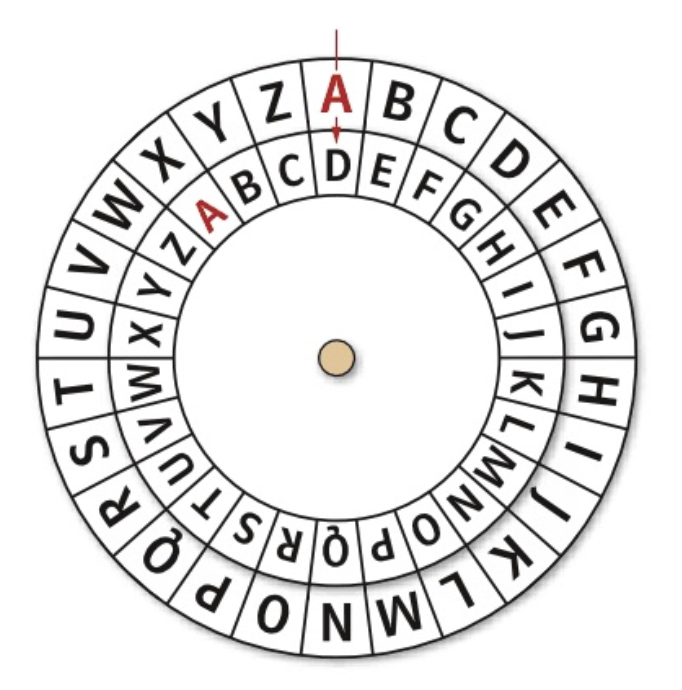
\includegraphics[width=\linewidth]{GrundlagenInfo/DataScience/03_Kryptologie/Figures/caesar.png}
    \end{figure}
    \end{minipage}
\end{frame}

\begin{frame}[label=multikey]{Kryptosystem mit vielen Schlüsseln}
  \begin{figure}[H]
        \centering
        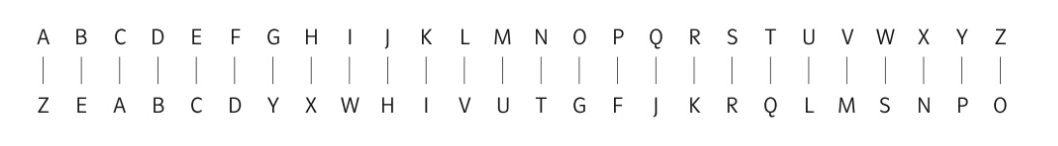
\includegraphics[width=\linewidth]{GrundlagenInfo/DataScience/03_Kryptologie/Figures/multikey.png}
    \end{figure}
    \textbf{Beispiel}: Der Text
    \begin{center}
        YCXCBCWICISCYLIBVZRRBWCVCLQCKCBCT
    \end{center}
    bedeutet:
    \begin{center}
        GEHEDEINENWEGUNDLASSDIELEUTEREDEN
    \end{center}
    Wie viele Schlüssel gibt es?
    \[26!=26\cdot25\cdot24\cdot...\cdot3\cdot2\cdot1=4.06\cdot 10^{26}\]
\end{frame}

\begin{frame}[fragile, label=hauefigkeit]{Häufigkeitsverteilung}
    \textbf{Problem}: All diese Kryptosysteme lassen sich mit einfacher Häufigkeitsanalyse knacken
    \begin{figure}[H]
        \centering
        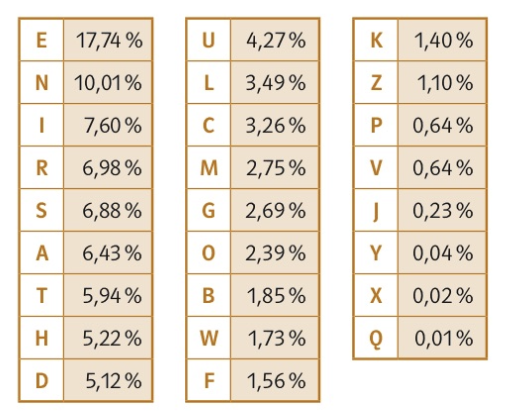
\includegraphics[width=.55\linewidth]{GrundlagenInfo/DataScience/03_Kryptologie/Figures/freq.png}
        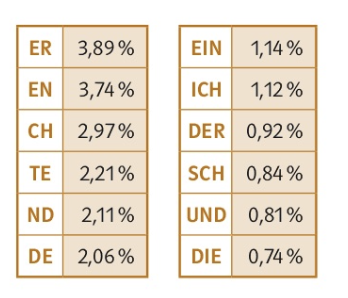
\includegraphics[width=.4\linewidth]{GrundlagenInfo/DataScience/03_Kryptologie/Figures/bigramme.png}
    \end{figure}

\defverbatim{\verbOne}{
\[h_\square (T)\]
= Häufigkeit von Buchstabe $\square$ in Text $T$.}
    
    \defverbatim{\verbTwo}{
    \begin{verbatim}
MUMMUXJUQYMHQUSUIUENGWTJEVHUMXRUQIMUMSUVYPPUM
----------------------------------------------
    \end{verbatim}
    U kommt 11-mal vor, M kommt 9-mal vor, Q kommt 6-mal vor}
    \defverbatim{\verbThree}{\small
    \begin{verbatim}
MUMMUXJUQYMHQOUSUTUQNGWTJQVHUMXQUQTMUMSUVYPPUM
NENNE--EI-N-I-E-E-EI-----I--EN-IEI-NEN-E----EN
    \end{verbatim}
    U kommt 11-mal vor, M kommt 9-mal vor, Q kommt 6-mal vor
    }
    
    \defverbatim{\verbFour}{\small\begin{verbatim}
MUMMUXJUQYMHQOUSUTUQNGWTJQVHUMXQUQTMUMSUVYPPUM
NENNEDREI-N-I-EGEHEI-----I--ENDIEIHNEN-E----EN 
    \end{verbatim}
    (Schlüssellänge=21 bzw. 5)}

    \defverbatim{\verbFive}{\small\begin{verbatim}
MUMMU|XJUQ|YMHQOUSUTUQNGWTJQVHUMXQUQTMUMSUVYPPUM
NENNE|DREI|-N-I-EGEHEI-----I--ENDIEIHNEN-E----EN 
    \end{verbatim}
    Man beginnt einige Wörter zu erkennen...}

    \defverbatim{\verbSix}{\small\begin{verbatim}
MUMMU|XJUQ|YMHQOU|SUTUQNGWTJQVHUM|XQU|QTM|UMSUVYPPUM
NENNE|DREI|-N-I-E|GEHEIMSCHRIFTEN|DIE|IHNEN|TE----EN 
    \end{verbatim}
    ``Geheimschriften?''}

    \defverbatim{\verbSeven}{\small\begin{verbatim}
MUMMU|XJUQ|YMHQOU|SUTUQNGWTJQVHUM|XQU|QTMUM|SUVYPPUM
NENNE|DREI|ANTIKE|GEHEIMSCHRIFTEN|DIE|IHNEN|GEFALLEN 
    \end{verbatim}
    \emoji{blush}}
    
    \only<1>{\verbOne}
    \only<2>{\verbTwo}
    \only<3>{\verbThree}
    \only<4>{\verbFour}
    \only<5>{\verbFive}
    \only<6>{\verbSix}
    \only<7>{\verbSeven}
\end{frame}

\begin{frame}[label=auftrag]{Auftrag}
\begin{itemize}
    \item \emoji{pen} Lesen Sie ``Neue Konzepte und Begriffe'' auf S. 59
    \item Aufgabe 2.16 (Tipp: Drehscheibe verwenden)
    \item Aufgabe 2.22
    %\item Aufgabe 2.29 (mit dem Computer)
    \item \emoji{trophy} Challenge: 
    \begin{itemize}
        \item Aufgabe 2.2 (\emoji{snake} Python)
        \item Aufgaben 2.3, 2.5 (\emoji{snake} Python)
        \item Aufgabe 2.19
    \end{itemize}
\end{itemize}
\end{frame}
\begin{frame}[label=summary]{Zusammenfassung}
\begin{itemize}[<+->]
    \item Verschlüsselung betrifft viele persönliche, soziale sowie politische Bereiche
    \item Daten sollen verschlüsselt übertragen werden, um Einblick durch fremde Personen zu vermeiden (Vertraulichkeit, Integrität, Authentizität, Verbindlichkeit)
    \item Mono- sowie polyalphabetische Kryptosysteme sind einfach zu knacken $\rightarrow$ Häufigkeitsanalyse (nächstes Mal)!
\end{itemize}
\end{frame}